\documentclass[12pt, letterpaper]{article}
\usepackage[includehead, margin=0.75in]{geometry}
\usepackage{fancyhdr}
\usepackage[british]{babel}
\usepackage{sansmathfonts}
\usepackage{tikz}
\usepackage{ifpdf}
\usepackage{soul}
\usepackage{color}
\usepackage{colortbl}
\usepackage{lewis}
\usepackage{siunitx}
\usepackage{textgreek}
\usepackage{mhchem}
\usepackage{modiagram}
\usepackage{tikzorbital}
\usepackage{chemfig}
\usepackage{xspace}
\definecolor{error}{rgb}{255,255,0}
\newcommand{\degree}{\ensuremath{{}^{\circ}}\xspace}
\renewcommand{\familydefault}{\sfdefault}


\usetikzlibrary{shapes,calc}

\ifpdf
  %
\else
  % Implement Outline text using pstricks if regular LaTeX->dvi->ps->pdf route
  \usepackage{pst-all}
\fi

\begin{document}

\newcommand{\CommonElementTextFormat}[4]
{
  \begin{minipage}{2.2cm}
    \centering
      {\textbf{#1} \hfill #2}%
      \linebreak \linebreak
      {\textbf{#3}}%
      \linebreak \linebreak
      {{#4}}
  \end{minipage}
}

\newcommand{\NaturalElementTextFormat}[4]
{
  \CommonElementTextFormat{#1}{#2}{\LARGE {#3}}{#4}
}

\newcommand{\OutlineText}[1]
{
\ifpdf
  % Couldn't find a nicer way of doing an outline font with TikZ
  % other than using pdfliteral 1 Tr
  %
  \pdfliteral direct {0.5 w 1 Tr}{#1}%
  \pdfliteral direct {1 w 0 Tr}%
\else
  % pstricks can do this with \pscharpath from pstricks
  %
  \pscharpath[shadow=false,
    fillstyle=solid,
    fillcolor=white,
    linestyle=solid,
    linecolor=black,
    linewidth=.2pt]{#1} 
\fi
}

\newcommand{\SyntheticElementTextFormat}[4]
{
\ifpdf
  \CommonElementTextFormat{#1}{#2}{\textsc{\LARGE #3}}{#4}
\else
  % pstricks approach results in slightly larger box
  % that doesn't break, so fudge here
  \CommonElementTextFormat{#1}{#2}{\textsc{\Large #3}}{#4}
\fi
}






\begin{document}

\fancypagestyle{plain}{%
  \fancyhf{}
  \fancyhead[L]{CHEM 112 - M01 \\ Dr. Moulder}
  \fancyhead[R]{H. Ryott Glayzer \\ \today}
  \fancyhead[C]{\large{Exam II Makeup Questions}\\ \;}
}

\title{Exam II Makeup Questions}
\author{H. Ryott Glayzer}
\date{\today}


\maketitle


\section*{Notice of ADA Accommodation and Methods}
I have an ADA accommodation to do my assignment on paper.
This document is a utilization of that accommodation.
This assignment will utilize the makeup questions for 
Exam II provided by Dr.\ Moulder.
Reasoning will be provided within the context of this
class, and at times, within the context of concepts
outside of the scope of this class.
Each problem will appear on a new page.

\bigskip
\\
\bigskip
\\
\bigskip
\\
\bigskip
\\

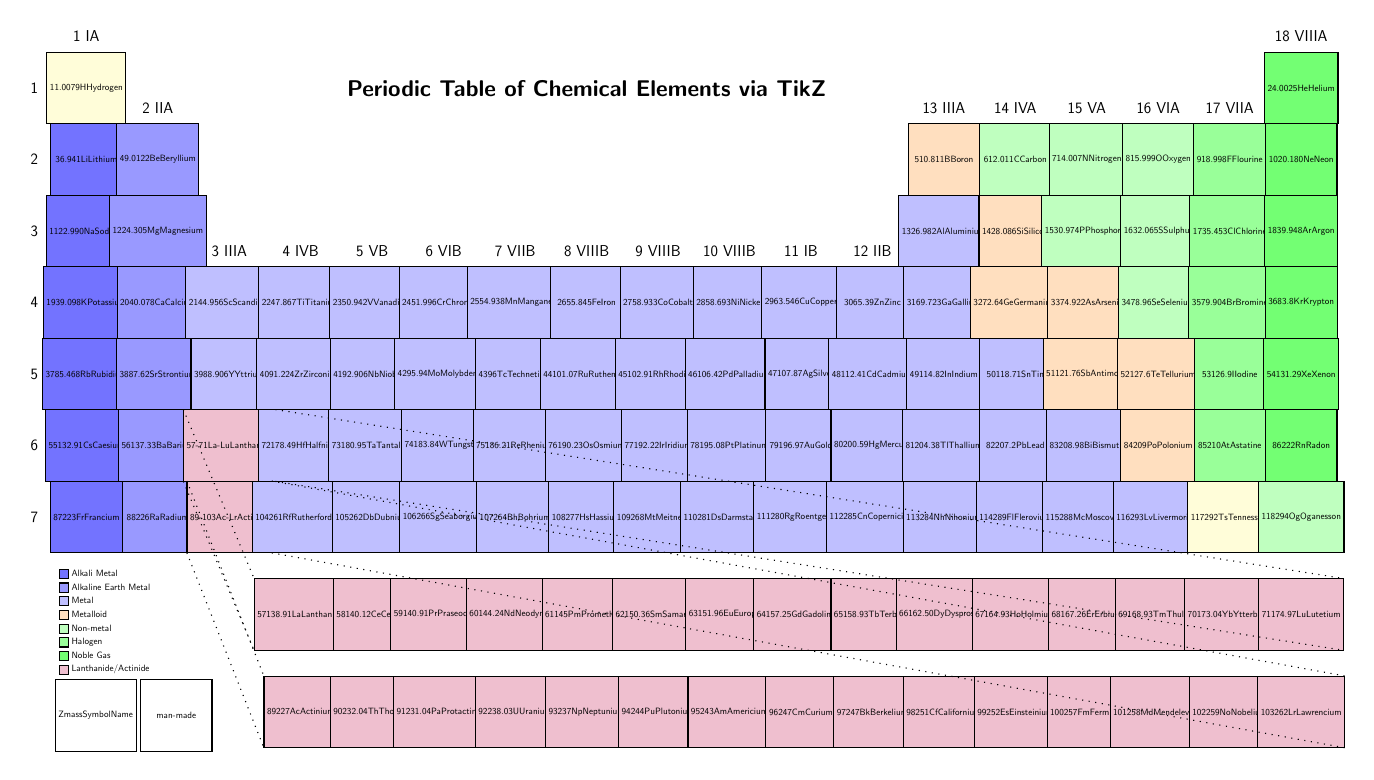
\begin{tikzpicture}[font=\sffamily, scale=0.33, transform shape]

%% Fill Color Styles
  \tikzstyle{ElementFill} = [fill=yellow!15]
  \tikzstyle{AlkaliMetalFill} = [fill=blue!55]
  \tikzstyle{AlkalineEarthMetalFill} = [fill=blue!40]
  \tikzstyle{MetalFill} = [fill=blue!25]
  \tikzstyle{MetalloidFill} = [fill=orange!25]
  \tikzstyle{NonmetalFill} = [fill=green!25]
  \tikzstyle{HalogenFill} = [fill=green!40]
  \tikzstyle{NobleGasFill} = [fill=green!55]
  \tikzstyle{LanthanideActinideFill} = [fill=purple!25]

%% Element Styles
  \tikzstyle{Element} = [draw=black, ElementFill,
    minimum width=2.75cm, minimum height=2.75cm, node distance=2.75cm]
  \tikzstyle{AlkaliMetal} = [Element, AlkaliMetalFill]
  \tikzstyle{AlkalineEarthMetal} = [Element, AlkalineEarthMetalFill]
  \tikzstyle{Metal} = [Element, MetalFill]
  \tikzstyle{Metalloid} = [Element, MetalloidFill]
  \tikzstyle{Nonmetal} = [Element, NonmetalFill]
  \tikzstyle{Halogen} = [Element, HalogenFill]
  \tikzstyle{NobleGas} = [Element, NobleGasFill]
  \tikzstyle{LanthanideActinide} = [Element, LanthanideActinideFill]
  \tikzstyle{PeriodLabel} = [font={\sffamily\LARGE}, node distance=2.0cm]
  \tikzstyle{GroupLabel} = [font={\sffamily\LARGE}, minimum width=2.75cm, node distance=2.0cm]
  \tikzstyle{TitleLabel} = [font={\sffamily\Huge\bfseries}]

%% Group 1 - IA
  \node[name=H, Element] {\NaturalElementTextFormat{1}{1.0079}{H}{Hydrogen}};
  \node[name=Li, below of=H, AlkaliMetal] {\NaturalElementTextFormat{3}{6.941}{Li}{Lithium}};
  \node[name=Na, below of=Li, AlkaliMetal] {\NaturalElementTextFormat{11}{22.990}{Na}{Sodium}};
  \node[name=K, below of=Na, AlkaliMetal] {\NaturalElementTextFormat{19}{39.098}{K}{Potassium}};
  \node[name=Rb, below of=K, AlkaliMetal] {\NaturalElementTextFormat{37}{85.468}{Rb}{Rubidium}};
  \node[name=Cs, below of=Rb, AlkaliMetal] {\NaturalElementTextFormat{55}{132.91}{Cs}{Caesium}};
  \node[name=Fr, below of=Cs, AlkaliMetal] {\NaturalElementTextFormat{87}{223}{Fr}{Francium}};

%% Group 2 - IIA
  \node[name=Be, right of=Li, AlkalineEarthMetal] {\NaturalElementTextFormat{4}{9.0122}{Be}{Beryllium}};
  \node[name=Mg, below of=Be, AlkalineEarthMetal] {\NaturalElementTextFormat{12}{24.305}{Mg}{Magnesium}};
  \node[name=Ca, below of=Mg, AlkalineEarthMetal] {\NaturalElementTextFormat{20}{40.078}{Ca}{Calcium}};
  \node[name=Sr, below of=Ca, AlkalineEarthMetal] {\NaturalElementTextFormat{38}{87.62}{Sr}{Strontium}};
  \node[name=Ba, below of=Sr, AlkalineEarthMetal] {\NaturalElementTextFormat{56}{137.33}{Ba}{Barium}};
  \node[name=Ra, below of=Ba, AlkalineEarthMetal] {\NaturalElementTextFormat{88}{226}{Ra}{Radium}};

%% Group 3 - IIIB
  \node[name=Sc, right of=Ca, Metal] {\NaturalElementTextFormat{21}{44.956}{Sc}{Scandium}};
  \node[name=Y, below of=Sc, Metal] {\NaturalElementTextFormat{39}{88.906}{Y}{Yttrium}};
  \node[name=LaLu, below of=Y, LanthanideActinide] {\NaturalElementTextFormat{57-71}{}{La-Lu}{Lanthanide}};
  \node[name=AcLr, below of=LaLu, LanthanideActinide] {\NaturalElementTextFormat{89-103}{}{Ac-Lr}{Actinide}};

%% Group 4 - IVB
  \node[name=Ti, right of=Sc, Metal] {\NaturalElementTextFormat{22}{47.867}{Ti}{Titanium}};
  \node[name=Zr, below of=Ti, Metal] {\NaturalElementTextFormat{40}{91.224}{Zr}{Zirconium}};
  \node[name=Hf, below of=Zr, Metal] {\NaturalElementTextFormat{72}{178.49}{Hf}{Halfnium}};
  \node[name=Rf, below of=Hf, Metal] {\SyntheticElementTextFormat{104}{261}{Rf}{Rutherfordium}};

%% Group 5 - VB
  \node[name=V, right of=Ti, Metal] {\NaturalElementTextFormat{23}{50.942}{V}{Vanadium}};
  \node[name=Nb, below of=V, Metal] {\NaturalElementTextFormat{41}{92.906}{Nb}{Niobium}};
  \node[name=Ta, below of=Nb, Metal] {\NaturalElementTextFormat{73}{180.95}{Ta}{Tantalum}};
  \node[name=Db, below of=Ta, Metal] {\SyntheticElementTextFormat{105}{262}{Db}{Dubnium}};

%% Group 6 - VIB
  \node[name=Cr, right of=V, Metal] {\NaturalElementTextFormat{24}{51.996}{Cr}{Chromium}};
  \node[name=Mo, below of=Cr, Metal] {\NaturalElementTextFormat{42}{95.94}{Mo}{Molybdenum}};
  \node[name=W, below of=Mo, Metal] {\NaturalElementTextFormat{74}{183.84}{W}{Tungsten}};
  \node[name=Sg, below of=W, Metal] {\SyntheticElementTextFormat{106}{266}{Sg}{Seaborgium}};

%% Group 7 - VIIB
  \node[name=Mn, right of=Cr, Metal] {\NaturalElementTextFormat{25}{54.938}{Mn}{Manganese}};
  \node[name=Tc, below of=Mn, Metal] {\NaturalElementTextFormat{43}{96}{Tc}{Technetium}};
  \node[name=Re, below of=Tc, Metal] {\NaturalElementTextFormat{75}{186.21}{Re}{Rhenium}};
  \node[name=Bh, below of=Re, Metal] {\SyntheticElementTextFormat{107}{264}{Bh}{Bohrium}};

%% Group 8 - VIIIB
  \node[name=Fe, right of=Mn, Metal] {\NaturalElementTextFormat{26}{55.845}{Fe}{Iron}};
  \node[name=Ru, below of=Fe, Metal] {\NaturalElementTextFormat{44}{101.07}{Ru}{Ruthenium}};
  \node[name=Os, below of=Ru, Metal] {\NaturalElementTextFormat{76}{190.23}{Os}{Osmium}};
  \node[name=Hs, below of=Os, Metal] {\SyntheticElementTextFormat{108}{277}{Hs}{Hassium}};

%% Group 9 - VIIIB
  \node[name=Co, right of=Fe, Metal] {\NaturalElementTextFormat{27}{58.933}{Co}{Cobalt}};
  \node[name=Rh, below of=Co, Metal] {\NaturalElementTextFormat{45}{102.91}{Rh}{Rhodium}};
  \node[name=Ir, below of=Rh, Metal] {\NaturalElementTextFormat{77}{192.22}{Ir}{Iridium}};
  \node[name=Mt, below of=Ir, Metal] {\SyntheticElementTextFormat{109}{268}{Mt}{Meitnerium}};

%% Group 10 - VIIIB
  \node[name=Ni, right of=Co, Metal] {\NaturalElementTextFormat{28}{58.693}{Ni}{Nickel}};
  \node[name=Pd, below of=Ni, Metal] {\NaturalElementTextFormat{46}{106.42}{Pd}{Palladium}};
  \node[name=Pt, below of=Pd, Metal] {\NaturalElementTextFormat{78}{195.08}{Pt}{Platinum}};
  \node[name=Ds, below of=Pt, Metal] {\SyntheticElementTextFormat{110}{281}{Ds}{Darmstadtium}};

%% Group 11 - IB
  \node[name=Cu, right of=Ni, Metal] {\NaturalElementTextFormat{29}{63.546}{Cu}{Copper}};
  \node[name=Ag, below of=Cu, Metal] {\NaturalElementTextFormat{47}{107.87}{Ag}{Silver}};
  \node[name=Au, below of=Ag, Metal] {\NaturalElementTextFormat{79}{196.97}{Au}{Gold}};
  \node[name=Rg, below of=Au, Metal] {\SyntheticElementTextFormat{111}{280}{Rg}{Roentgenium}};

%% Group 12 - IIB
  \node[name=Zn, right of=Cu, Metal] {\NaturalElementTextFormat{30}{65.39}{Zn}{Zinc}};
  \node[name=Cd, below of=Zn, Metal] {\NaturalElementTextFormat{48}{112.41}{Cd}{Cadmium}};
  \node[name=Hg, below of=Cd, Metal] {\NaturalElementTextFormat{80}{200.59}{Hg}{Mercury}};
  \node[name=Uub, below of=Hg, Metal] {\SyntheticElementTextFormat{112}{285}{Cn}{Copernicium}};

%% Group 13 - IIIA
  \node[name=Ga, right of=Zn, Metal] {\NaturalElementTextFormat{31}{69.723}{Ga}{Gallium}};
  \node[name=Al, above of=Ga, Metal] {\NaturalElementTextFormat{13}{26.982}{Al}{Aluminium}};
  \node[name=B, above of=Al, Metalloid] {\NaturalElementTextFormat{5}{10.811}{B}{Boron}};
  \node[name=In, below of=Ga, Metal] {\NaturalElementTextFormat{49}{114.82}{In}{Indium}};
  \node[name=Tl, below of=In, Metal] {\NaturalElementTextFormat{81}{204.38}{Tl}{Thallium}};
  \node[name=Uut, below of=Tl, Metal] {\SyntheticElementTextFormat{113}{284}{Nh}{Nihonium}};

%% Group 14 - IVA
  \node[name=C, right of=B, Nonmetal] {\NaturalElementTextFormat{6}{12.011}{C}{Carbon}};
  \node[name=Si, below of=C, Metalloid] {\NaturalElementTextFormat{14}{28.086}{Si}{Silicon}};
  \node[name=Ge, below of=Si, Metalloid] {\NaturalElementTextFormat{32}{72.64}{Ge}{Germanium}};
  \node[name=Sn, below of=Ge, Metal] {\NaturalElementTextFormat{50}{118.71}{Sn}{Tin}};
  \node[name=Pb, below of=Sn, Metal] {\NaturalElementTextFormat{82}{207.2}{Pb}{Lead}};
  \node[name=Uuq, below of=Pb, Metal] {\SyntheticElementTextFormat{114}{289}{Fl}{Flerovium}};

%% Group 15 - VA
  \node[name=N, right of=C, Nonmetal] {\NaturalElementTextFormat{7}{14.007}{N}{Nitrogen}};
  \node[name=P, below of=N, Nonmetal] {\NaturalElementTextFormat{15}{30.974}{P}{Phosphorus}};
  \node[name=As, below of=P, Metalloid] {\NaturalElementTextFormat{33}{74.922}{As}{Arsenic}};
  \node[name=Sb, below of=As, Metalloid] {\NaturalElementTextFormat{51}{121.76}{Sb}{Antimony}};
  \node[name=Bi, below of=Sb, Metal] {\NaturalElementTextFormat{83}{208.98}{Bi}{Bismuth}};
  \node[name=Uup, below of=Bi, Metal] {\SyntheticElementTextFormat{115}{288}{Mc}{Moscovium}};

%% Group 16 - VIA
  \node[name=O, right of=N, Nonmetal] {\NaturalElementTextFormat{8}{15.999}{O}{Oxygen}};
  \node[name=S, below of=O, Nonmetal] {\NaturalElementTextFormat{16}{32.065}{S}{Sulphur}};
  \node[name=Se, below of=S, Nonmetal] {\NaturalElementTextFormat{34}{78.96}{Se}{Selenium}};
  \node[name=Te, below of=Se, Metalloid] {\NaturalElementTextFormat{52}{127.6}{Te}{Tellurium}};
  \node[name=Po, below of=Te, Metalloid] {\NaturalElementTextFormat{84}{209}{Po}{Polonium}};
  \node[name=Uuh, below of=Po, Metal] {\SyntheticElementTextFormat{116}{293}{Lv}{Livermorium}};

%% Group 17 - VIIA
  \node[name=F, right of=O, Halogen] {\NaturalElementTextFormat{9}{18.998}{F}{Flourine}};
  \node[name=Cl, below of=F, Halogen] {\NaturalElementTextFormat{17}{35.453}{Cl}{Chlorine}};
  \node[name=Br, below of=Cl, Halogen] {\NaturalElementTextFormat{35}{79.904}{Br}{Bromine}};
  \node[name=I, below of=Br, Halogen] {\NaturalElementTextFormat{53}{126.9}{I}{Iodine}};
  \node[name=At, below of=I, Halogen] {\NaturalElementTextFormat{85}{210}{At}{Astatine}};
  \node[name=Uus, below of=At, Element] {\SyntheticElementTextFormat{117}{292}{Ts}{Tennessine}}; 

%% Group 18 - VIIIA
  \node[name=Ne, right of=F, NobleGas] {\NaturalElementTextFormat{10}{20.180}{Ne}{Neon}};
  \node[name=He, above of=Ne, NobleGas] {\NaturalElementTextFormat{2}{4.0025}{He}{Helium}};
  \node[name=Ar, below of=Ne, NobleGas] {\NaturalElementTextFormat{18}{39.948}{Ar}{Argon}};
  \node[name=Kr, below of=Ar, NobleGas] {\NaturalElementTextFormat{36}{83.8}{Kr}{Krypton}};
  \node[name=Xe, below of=Kr, NobleGas] {\NaturalElementTextFormat{54}{131.29}{Xe}{Xenon}};
  \node[name=Rn, below of=Xe, NobleGas] {\NaturalElementTextFormat{86}{222}{Rn}{Radon}};
  \node[name=Uuo, below of=Rn, Nonmetal] {\SyntheticElementTextFormat{118}{294}{Og}{Oganesson}}; 

%% Period
  \node[name=Period1, left of=H, PeriodLabel] {1};
  \node[name=Period2, left of=Li, PeriodLabel] {2};
  \node[name=Period3, left of=Na, PeriodLabel] {3}; 
  \node[name=Period4, left of=K, PeriodLabel] {4}; 
  \node[name=Period5, left of=Rb, PeriodLabel] {5};
  \node[name=Period6, left of=Cs, PeriodLabel] {6};
  \node[name=Period7, left of=Fr, PeriodLabel] {7};

%% Group
  \node[name=Group1, above of=H, GroupLabel] {1 \hfill IA};
  \node[name=Group2, above of=Be, GroupLabel] {2 \hfill IIA};
  \node[name=Group3, above of=Sc, GroupLabel] {3 \hfill IIIA};
  \node[name=Group4, above of=Ti, GroupLabel] {4 \hfill IVB};
  \node[name=Group5, above of=V, GroupLabel] {5 \hfill VB};
  \node[name=Group6, above of=Cr, GroupLabel] {6 \hfill VIB};
  \node[name=Group7, above of=Mn, GroupLabel] {7 \hfill VIIB};
  \node[name=Group8, above of=Fe, GroupLabel] {8 \hfill VIIIB};
  \node[name=Group9, above of=Co, GroupLabel] {9 \hfill VIIIB};
  \node[name=Group10, above of=Ni, GroupLabel] {10 \hfill VIIIB};
  \node[name=Group11, above of=Cu, GroupLabel] {11 \hfill IB};
  \node[name=Group12, above of=Zn, GroupLabel] {12 \hfill IIB};
  \node[name=Group13, above of=B, GroupLabel] {13 \hfill IIIA};
  \node[name=Group14, above of=C, GroupLabel] {14 \hfill IVA};
  \node[name=Group15, above of=N, GroupLabel] {15 \hfill VA};
  \node[name=Group16, above of=O, GroupLabel] {16 \hfill VIA};
  \node[name=Group17, above of=F, GroupLabel] {17 \hfill VIIA};
  \node[name=Group18, above of=He, GroupLabel] {18 \hfill VIIIA};

%% Lanthanide
  \node[name=La, below of=Rf, LanthanideActinide, yshift=-1cm] {\NaturalElementTextFormat{57}{138.91}{La}{Lanthanum}};
  \node[name=Ce, right of=La, LanthanideActinide] {\NaturalElementTextFormat{58}{140.12}{Ce}{Cerium}};
  \node[name=Pr, right of=Ce, LanthanideActinide] {\NaturalElementTextFormat{59}{140.91}{Pr}{Praseodymium}};
  \node[name=Nd, right of=Pr, LanthanideActinide] {\NaturalElementTextFormat{60}{144.24}{Nd}{Neodymium}};
  \node[name=Pm, right of=Nd, LanthanideActinide] {\NaturalElementTextFormat{61}{145}{Pm}{Promethium}};
  \node[name=Sm, right of=Pm, LanthanideActinide] {\NaturalElementTextFormat{62}{150.36}{Sm}{Samarium}};
  \node[name=Eu, right of=Sm, LanthanideActinide] {\NaturalElementTextFormat{63}{151.96}{Eu}{Europium}};
  \node[name=Gd, right of=Eu, LanthanideActinide] {\NaturalElementTextFormat{64}{157.25}{Gd}{Gadolinium}};
  \node[name=Tb, right of=Gd, LanthanideActinide] {\NaturalElementTextFormat{65}{158.93}{Tb}{Terbium}};
  \node[name=Dy, right of=Tb, LanthanideActinide] {\NaturalElementTextFormat{66}{162.50}{Dy}{Dysprosium}};
  \node[name=Ho, right of=Dy, LanthanideActinide] {\NaturalElementTextFormat{67}{164.93}{Ho}{Holmium}};
  \node[name=Er, right of=Ho, LanthanideActinide] {\NaturalElementTextFormat{68}{167.26}{Er}{Erbium}};
  \node[name=Tm, right of=Er, LanthanideActinide] {\NaturalElementTextFormat{69}{168.93}{Tm}{Thulium}};
  \node[name=Yb, right of=Tm, LanthanideActinide] {\NaturalElementTextFormat{70}{173.04}{Yb}{Ytterbium}};
  \node[name=Lu, right of=Yb, LanthanideActinide] {\NaturalElementTextFormat{71}{174.97}{Lu}{Lutetium}};

%% Actinide
  \node[name=Ac, below of=La, LanthanideActinide, yshift=-1cm] {\NaturalElementTextFormat{89}{227}{Ac}{Actinium}};
  \node[name=Th, right of=Ac, LanthanideActinide] {\NaturalElementTextFormat{90}{232.04}{Th}{Thorium}};
  \node[name=Pa, right of=Th, LanthanideActinide] {\NaturalElementTextFormat{91}{231.04}{Pa}{Protactinium}};
  \node[name=U, right of=Pa, LanthanideActinide] {\NaturalElementTextFormat{92}{238.03}{U}{Uranium}};
  \node[name=Np, right of=U, LanthanideActinide] {\SyntheticElementTextFormat{93}{237}{Np}{Neptunium}};
  \node[name=Pu, right of=Np, LanthanideActinide] {\SyntheticElementTextFormat{94}{244}{Pu}{Plutonium}};
  \node[name=Am, right of=Pu, LanthanideActinide] {\SyntheticElementTextFormat{95}{243}{Am}{Americium}};
  \node[name=Cm, right of=Am, LanthanideActinide] {\SyntheticElementTextFormat{96}{247}{Cm}{Curium}};
  \node[name=Bk, right of=Cm, LanthanideActinide] {\SyntheticElementTextFormat{97}{247}{Bk}{Berkelium}};
  \node[name=Cf, right of=Bk, LanthanideActinide] {\SyntheticElementTextFormat{98}{251}{Cf}{Californium}};
  \node[name=Es, right of=Cf, LanthanideActinide] {\SyntheticElementTextFormat{99}{252}{Es}{Einsteinium}};
  \node[name=Fm, right of=Es, LanthanideActinide] {\SyntheticElementTextFormat{100}{257}{Fm}{Fermium}};
  \node[name=Md, right of=Fm, LanthanideActinide] {\SyntheticElementTextFormat{101}{258}{Md}{Mendelevium}};
  \node[name=No, right of=Md, LanthanideActinide] {\SyntheticElementTextFormat{102}{259}{No}{Nobelium}};
  \node[name=Lr, right of=No, LanthanideActinide] {\SyntheticElementTextFormat{103}{262}{Lr}{Lawrencium}};

%% Draw dotted lines connecting Lanthanide breakout to main table
  \draw (LaLu.north west) edge[dotted] (La.north west)
        (LaLu.north east) edge[dotted] (Lu.north east)
        (LaLu.south west) edge[dotted] (La.south west)
        (LaLu.south east) edge[dotted] (Lu.south east);
%% Draw dotted lines connecting Actinide breakout to main table
  \draw (AcLr.north west) edge[dotted] (Ac.north west)
        (AcLr.north east) edge[dotted] (Lr.north east)
        (AcLr.south west) edge[dotted] (Ac.south west)
        (AcLr.south east) edge[dotted] (Lr.south east);

%% Legend
  \draw[black, AlkaliMetalFill] ($(La.north -| Fr.west) + (1em,-0.0em)$)
    rectangle +(1em, 1em) node[right, yshift=-1ex]{Alkali Metal};
  \draw[black, AlkalineEarthMetalFill] ($(La.north -| Fr.west) + (1em,-1.5em)$)
    rectangle +(1em, 1em) node[right, yshift=-1ex]{Alkaline Earth Metal};
  \draw[black, MetalFill] ($(La.north -| Fr.west) + (1em,-3.0em)$)
    rectangle +(1em, 1em) node[right, yshift=-1ex]{Metal};
  \draw[black, MetalloidFill] ($(La.north -| Fr.west) + (1em,-4.5em)$)
    rectangle +(1em, 1em) node[right, yshift=-1ex]{Metalloid};
  \draw[black, NonmetalFill] ($(La.north -| Fr.west) + (1em,-6.0em)$)
    rectangle +(1em, 1em) node[right, yshift=-1ex]{Non-metal};
  \draw[black, HalogenFill] ($(La.north -| Fr.west) + (1em,-7.5em)$)
    rectangle +(1em, 1em) node[right, yshift=-1ex]{Halogen};
  \draw[black, NobleGasFill] ($(La.north -| Fr.west) + (1em,-9.0em)$)
    rectangle +(1em, 1em) node[right, yshift=-1ex]{Noble Gas};
  \draw[black, LanthanideActinideFill] ($(La.north -| Fr.west) + (1em,-10.5em)$)
    rectangle +(1em, 1em) node[right, yshift=-1ex]{Lanthanide/Actinide};

  \node at ($(La.north -| Fr.west) + (5em,-15em)$) [name=elementLegend, Element, fill=white]
    {\NaturalElementTextFormat{Z}{mass}{Symbol}{Name}};
  \node[Element, fill=white, right of=elementLegend, xshift=1em]
    {\SyntheticElementTextFormat{}{}{man-made}{}} ;

%% Diagram Title
  \node at (H.west -| Fe.north) [name=diagramTitle, TitleLabel]
    {Periodic Table of Chemical Elements via Ti\emph{k}Z};

\end{tikzpicture}


\clearpage

\section*{Calculate the Velocity of Electrons with de Broglie Wavelengths of 285 nm.}

The equation 
\[
	\lambda = \frac{h}{mv}
\]
is accurate for non-relativistic velocities.
For relativistic velocities, the equation 
\[
	\frac{1}{\lambda_B} = \frac{mv}{h \sqrt{1-\frac{v^{2}}{c^{2}}}}
\]
is more accurate.
I will determine the velocity of electrons with de Broglie wavelengths of 285 nm 
using both of these equations.


\subsection*{Calculating the de Broglie Wavelength with the Non-Relativistic Equation}
For the non-relativistic equation, we will first consider that the mass of an electron
is given to be 9.1094 x 10$^{-31}$ kg.
The non-relativistic equation:
\[
	\lambda = \frac{h}{mv}
\]
can be rewritten:
\[
	h = mv\lambda.
\]
To determine the velocity, we can rearrange the equation to give the velocity:
\[
	v = \frac{h}{m\lambda}.
\]
Substituting the variables with known values, with the knowledge that
$\qty{1}{\joule} = \qty{1}{\kilo\gram\square\metre\per\square\second}$,
gives:
\[
	v = \frac
	{\qty[mode=text]{6.63e-34}{\kilo\gram\square\metre\per\square\second\second}}
	{\qty[mode=text]{9.1094e-31}{\kilo\gram}\times\qty[mode=text]{2.85e-7}{\metre}}.
\]
This gives:
\[
	v \unit{\metre\per\second} = \frac
	{\qty[mode=text]{6.63e-34}{\kilo\gram\square\metre\per\second}}
	{\qty[mode=text]{2.596179e-37}{\kilo\gram\metre}}
\]
which provides the value:
\[
	v = \qty{2.553753035e3}{\metre\per\second} = \qty{2.553e3}{\metre\per\second}
\]
This value is closest to multiple choice option 
\textbf{D: \qty[mode=text]{2.552e3}{\metre\per\second}}.

\subsection*{Calculating the de Broglie wavelength using the Proper Relativistic Equation}
The de Broglie wavelength of a particle is a wavelength that determines the probability
density of the particle being found at a specific point $q$ in its configuration space.
This is important in quantum mechanics. 
In the context of General Chemistry I, the de Broglie wavelength is defined in our 
textbook only as a characteristic of particles and other bodies.
The relativistic definition of the de Broglie wavelength is:
\[
	\lambda_B = \frac{h}{p},
\]
where $\lambda_B$ represents the de Broglie wavelength of the particle,
$h$ represents the Planck constant,
which has the value \SI{6.62607015e-34}{\joule\second},
and $p$ represents the relativistic momentum of the particle, defined as
\[
	p = \frac{mv}{\sqrt{1-\frac{v^{2}}{c^{2}}}},
\]
with $m$ representing the mass of the particle,
$v$ representing the particle's velocity, 
and $c$ representing the speed of light in a vacuum.
The invariant mass of the electron is approximately
$\SI{9.1093837015 \pm 0.0000000028 e-31}{\kilo\gram}$
according to the NIST\@.
The speed of light in a vacuum is defined as 
$\SI{299792458}{\metre\per\second}$.

Combining these equations gives the formula:
\[
	\lambda_B = \frac
	{h}
	{\frac{mv}{\sqrt{1-\frac{v^{2}}{c^{2}}}}}
\]
which simplifies to
\[
	\lambda_B = \frac
	{h\sqrt{1-\frac{v^{2}}{c^{2}}}}
	{mv}.
\]
This can be rearranged to 
\[
	\lambda_B m v = h \sqrt{1-\frac{v^{2}}{c^{2}}}.
\]
root -?
The following steps will solve the equation for velocity:
\[
	\frac{\lambda_B m v}{h} = \sqrt{1-\frac{v^2}{c^2}}
	\Rightarrow
	{(\frac{\lambda_B m v}{h})}^{2} = 
	{(\sqrt{1 - \frac{v^2}{c^2}})}^{2} 
	\Rightarrow
	\frac{\lambda_B^{2}m^{2}v^{2}}{h^{2}} = 1 - \frac{v^{2}}{c^{2}}
	\Rightarrow
\]
\\
\[
	1 = \frac{\lambda_B^2 m^2 v^2}{h^2} + \frac{v^2}{c^2}	
	\Rightarrow
	1 = \frac{\lambda_B^2 m^2 v^2 c^2 + v^2 h^2}{h^2 c^2}
	\Rightarrow
	h^2 c^2 = \lambda_B^2 m^2 v^2 c^2 + v^2 h^2
	\Rightarrow
\]
\\
\[
	h^2 c^2 = v^2 ( \lambda_B^2 m^2 c^2 + h^2 )
	\Rightarrow
	v^2 = \frac
	{h^2 c^2}
	{\lambda_B^2 m^2 c^2}
	\Rightarrow
	v = \sqrt{
		\frac{h^2 c^2}{\lambda_B^2 m^2 c^2}
	}
\]
\[
	v = \sqrt{
		\frac{h^2}{\lambda_B^2 m^2}
	}
\]
And thus, we have arrived at the relativistic equation for the
de Broglie wavelength solved for velocity.
Using the values we defined earlier, we find the velocity to be:
\[
	v^2 = 
	\frac
	{(\SI{6.62607015e-34}{\joule\second})^{2}}
	{(\SI{285e-9}{\metre})^{2} \times (\SI{9.1093837015e-31}{\kilo\gram})^{2}}
\]
\\
\[
	v^2 = \frac
	{\SI{4.390480563e-67}{\kilo\square\gram\metre^{4}\second^{-2}}}
	{\SI{6.740121281e-74}{\kilo\square\gram\square\metre}}
\]
\\
\[
	v^2 = \SI{6.513948904e6}{\square\metre\per\square\second}
\]
\\
\[
	v = \SI{2.552243896e3}{\metre\per\second},
\]
which, upon applying significant figures, would come to 
\[
	v = \SI{2.552e3}{\metre\per\second}
\]
This is exactly the multiple choice option \textbf{D}.

\subsection*{Solution}

Both the non-relativistic approximation and the true relativistic equation
give the answer 
\[
\textbf{D}.\quad \SI{2.552e3}{\metre\per\second}.
\]
\\
\\
\clearpage

\section*{What Element is Theoretically the Smallest of all on the Periodic Table?}
The smallest theoretical element is Helium.
This follows the periodic trends of atomic radius.
As an element's group grows, its radius shrinks as there are more electrons 
in its shell,
and the radius grows as the period increases,
as there are more electron shells.
Since Hydrogen has the most electrons and the least electron shells,
Helium is the smallest element.



\clearpage



\section*{What wavelength would the hydrogen Rydberg line give for the electronic
transition $n_1 = 2$ and $n_2 = 5$?}

The Rydberg formula models the emission and absorption wavelengths for 
photons in jumps in electron energy levels. It is defined for hydrogen as follows:

\[
	\frac{1}{\lambda_{vac}} = R_H\left(\frac{1}{n_1^2}-\frac{1}{n_2^2}\right)
\]
where $R_H$ is defined in the handout as \SI{1.097e7}{\per\metre}.
This gives us the equation
\[
	\frac{1}{\lambda_{vac}} = \left(\SI{1.097e7}{\per\metre}\right)
	\left( \frac{1}{n_1^2} - \frac{1}{n_2^2}  \right)
\]

The problem is asking for the Rydberg line for $n_1$ = 2 and $n_2$ = 5.
Plugging these into the formula gives us 
\[
	\frac{1}{\lambda_{vac}} = 
	\left(
		\SI{1.097e7}{\per\metre}
		\right)
		\left(
		\frac{1}{4} - \frac{1}{25}
			\right)
\]
Fraction Subtraction rules tell us that we need to find a common denominator.
\[
	\frac{1}{\lambda_{vac}} = R_H
	\left( 
		\frac{25}{100} - \frac{4}{100}	
	\right)
	= R_H \left(
		\frac{21}{100}
		\right)
\]
From this, we can see that 
\[
	\lambda_{vac} = \frac{100}{21 \times \SI{1.097e7}{\per\metre}}
\]

Which gives us 
\[
	\lambda_{vac} = \SI{4.341e-7}{\metre}
\]
which is approximately equal to \SI{434.0}{\nano\metre}.
\\
\\
Thus, the wavelength of the hydrogen Rydberg line for the electronic
transition from 2 to 5 would be \SI{434.0}{\nano\metre}, or multiple
choice option \textbf{C}.



\clearpage
\section*{Which is the most correct Lewis structure for \ce{N2O}}

Both Nitrogen and Oxygen in \ce{N2O} can be the central atom, so we determine
the central atom by determining the least electronegative atom and placing it
in the middle.
\ce{N} has electronegativity 3.04, while \ce{O} has electronegativity 3.44.
Thus, Nitrogen will be the central atom.
\\
There are five valence electrons in each nitrogen atom, and six in the oxygen
atom. 
Thus, there are sixteen total valence electrons in \ce{N2O}.
\\
Next, we must draw the skeleton structure for \ce{N2O}.
\begin{center}
	\chemfig{\lewis{N}{.}{.}{.}{}{.}{}{.}{}\lewis{N}{.}{.}{.}{}{.}{}{.}{}\lewis{O}{.}{.}{.}{}{.}{.}{.}{}}
\end{center}
\\
Now, we connect each atom with the central atom with a single bond.
\begin{center}
	\chemfig{\lewis{N}{.}{.}{.}{}{}{}{.}{}-\lewis{N}{}{}{.}{.}{}{}{}{.}-\lewis{O}{}{}{.}{.}{.}{}{.}{.}}
\end{center}
\\
Now, we must create new bonds in the central atom to create double and triple bonds.
\begin{center}
	\chemfig{\lewis{N}{.}{.}{}{}{}{}{}{}=\lewis{N}{}{}{.}{.}{}{}{}{}=\lewis{O}{}{}{.}{.}{}{}{.}{.}}
\end{center}
\\
The \ce{N} atom on the end does not follow the octet rule. 
Thus, we must move around bonds to make it valid.
\begin{center}
	\chemfig{\lewis{N}{.}{.}{}{}{}{}{}{}~N-\lewis{O}{}{}{.}{.}{.}{.}{.}{.}}
\end{center}
\\
This works, but there are resonance structures:
\begin{center}
	\chemfig{\lewis{N}{.}{.}{.}{.}{}{}{.}{.}-N~\lewis{O}{}{}{}{}{.}{.}{}{}}
\end{center}
\\
and
\begin{center}
	\chemfig{\lewis{N}{}{}{.}{.}{}{}{.}{.}=N=\lewis{O}{}{}{.}{.}{}{}{.}{.}}
\end{center}
\\
Now, we must compute the formal charges of each of the above resonance structures.
Formal Charge can be calculated via the following
\[
  \textbf{Q}_{\textup{Formal}} = \textbf{V}_{e^{-}} - \textbf{LP}_{e^{-}} - \frac{\textbf{B}_{e^-}}{2}
\]
\\
For the first structure, \chemfig{N~N-O}, the Formal Charge is computed:
\[
  \textbf{N}_{edge}: 5 - 2 - \frac{6}{2} = 0
\]

\[
\textbf{N}_{central}: 5 - 0 - \frac{8}{2} = +1
\]
\[
  \textbf{O}: 6 - 6 - \frac{2}{2} = -1
\]
Thus the formal charge of the first resonance structure, \chemfig{N~N-O}, is 
$0+1-1=0$.
This has the negative charge on the Oxygen and the positive charge on the Nitrogen.
The Oxygen is the more electronegative of the two, so this is the most correct
structure for \ce{N2O}:
\begin{center}
  \chemfig{\lewis{N}{.}{.}{}{}{}{}{}{}~N-\lewis{O}{}{}{.}{.}{.}{.}{.}{.}}
\end{center}
\\
This version is close to multiple choice option \textbf{D}.

\clearpage
\section*{What is the Frequency of Light that has a wavelength of 185 nm?}

The frequency of a photon can be derived in a classical sense through
\[
  \lambda = \frac{\textup{c}}{\nu}
\]
as such
\[
\nu = \frac{c}{\lambda}
\]
We can input the necessary values for $c$ and $\lambda$.
\[
  \nu = \frac{\SI{3.00e8}{\metre\per\second}}{\SI{185e-9}{\metre}}
\]
this gives us the value
\[
  \nu = \SI{1.62e15}{\per\second}
\]
This is the value of the multiple choice option \textbf{E}.





\clearpage
\section*{Which element is most likely to present with the first five
ionization energies specified below? (in \unit{\kilo\joule\per\mole})}
\begin{center}
	\begin{tabular}{|c|c|c|c|c|}
		\hline 
		\large{589.8} & \large{1145} & \large{4912} & \large{6491} & \large{8153} \\
		\hline
	\end{tabular}	
\end{center}
\\
\\

These five ionization energies are increasing in order.
Since the third ionization energy is exhibits a great increase, and it is greatly 
difficult to remove an electron from a full octet, one can assume that the atom
has two valence electrons.
Looking at the provided options, the only group 2 element in Calcium.
Thus, one can assume the answer is Calcium, multiple choice option \textbf{B}.


\clearpage
\section*{What is the hybridization of all the carbon atoms in benzene (\ce{C6H6})?}


























\clearpage
\section*{Based on their electronic configurations, which of the following elements 
or ions is paramagnetic in a vapor phase?}



























\clearpage
\section*{What is the maximum number of electrons that can have the following set of 
quantum numbers: n = 4, l = 3 $m_l$ = 3, $m_s$ = $-\frac{1}{2}$}

























\clearpage
\section*{Order the following series of isoelectronic ions 
(\ce{Mg^2+}, \ce{N^3-}, \ce{F-}, \ce{Si^4+}) from largest to smallest ionic
radii.}





































\end{document}





%%%%%%%%%%%%%%%%%%%%%%%%%%%%%%%%%%%%%%%%%%%%%%%%%%%%%%%%%%%%%%%%%%%%%%%%%%%%%%%
%%%                                 Copypasta                               %%%
%%%%%%%%%%%%%%%%%%%%%%%%%%%%%%%%%%%%%%%%%%%%%%%%%%%%%%%%%%%%%%%%%%%%%%%%%%%%%%%

% Table for questions with multiple parts

% \begin{center}
% 	\begin{tabular}{|c|c|c|c|c|}
% 		\hline
% 		_ & _ & _ & _ & _ \\
% 		\hline
% 		_ & _ & _ & _ & _ \\
% 		\hline
% 	\end{tabular}
% \end{center}
